When presented a motion sequence, moving hand is first detected in each image of the sequence. This is done in a number of steps.

At first image background is subtracted from the image. This allows us to only see things which have changed comparing to the background. Example of image from which background was subtracted is shown in Figure \ref{fig:bgsub}.

\begin{figure}
\begin{center}
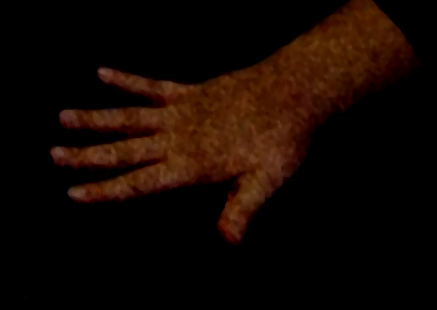
\includegraphics[width=80mm]{bgsub.png}
\caption{Image obtained by performing background subtraction.}
\label{fig:bgsub}
\end{center}
\end{figure}


Obtained image is then smoothened using median blur in order to reduce noise. Such image is then transformed into black and white image according to threshold based on a colour of a typical hand in the data set. Such colour is found to lie between RGB values of $(0, 0, 27)$ and $(100, 100, 140)$. Image obtained by thresholding is shown in Figure \ref{fig:bw}.

\begin{figure}
\begin{center}
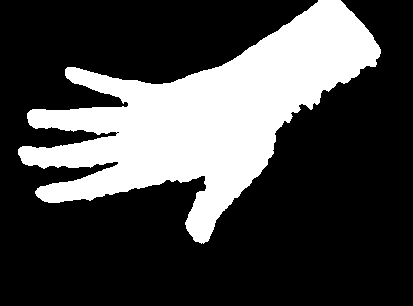
\includegraphics[width=80mm]{bw.png}
\caption{Image obtained by thresholding preprocessed image.}
\label{fig:bw}
\end{center}
\end{figure}


To improve precision of the background subtraction and to account for possible lighting changes between different sets of images, first image of the sequence is also subtracted from the image. This removes all static features from the image. Such static features are often artifacts caused by changed lighting conditions. Both, first image which is subtracted from image of interest and image of interest itself, are preprocessed in the same way.

\begin{math}
Image^*_n = f(Image_n - Background) - f(Image_1 - Background), n \geq 2
\end{math}

Erosion and dilation is then done for such image. This helps further smoothen the detected hand and also helps eradicate any noise which appears not attached to the hand.

Contours of the objects are then detected using simple chain approximation algorithm. Such algorithm scans binary image vertically as well as horizontally looking for chains of white pixels. It flips all the white pixels except from the pixels which represent both ends of each such chain. Using this technique we are able to obtain contours of all objects in the image. Contours of object obtained by using this method is showin in Figure \ref{fig:contours}.

\begin{figure}
\begin{center}
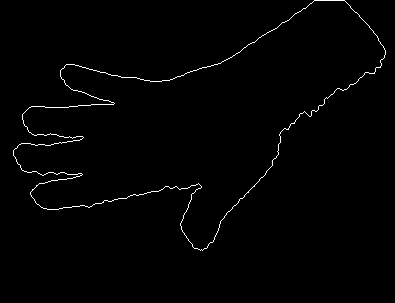
\includegraphics[width=80mm]{contours.png}
\caption{Image obtained by using simple chain approximation algorithm.}
\label{fig:contours}
\end{center}
\end{figure}

Largest object in the image is then chosen. If area of such object is above given threshold, the object is chosen as representation of the hand in the image.